\documentclass[prb,aps,twocolumn,showpacs,10pt]{revtex4-1}
\pdfoutput=1
\usepackage{dcolumn}% Align table columns on decimal point
\usepackage{bm}% bold math

%\usepackage{anysize}
\usepackage[colorlinks,hyperindex, urlcolor=blue, linkcolor=blue,citecolor=black, linkbordercolor={.7 .8 .8}]{hyperref}
\usepackage{graphicx}
%\usepackage{tabularx}
\usepackage{amsfonts}
\usepackage{amsmath}
\usepackage{amssymb}
\usepackage{amsbsy}
\usepackage{tikz}
%\usepackage{wrapfig}
%\usepackage{setspace}
%\usepackage{caption}
%\usepackage{fancyhdr}
\usepackage{nicefrac}
\usetikzlibrary{arrows,shapes,positioning}
\newenvironment{psmallmatrix}
  {\left[\begin{matrix}}
  {\end{matrix}\right]}
  
 \usepackage{listings}
\usepackage{color}

\definecolor{dkgreen}{rgb}{0,0.6,0}
\definecolor{gray}{rgb}{0.5,0.5,0.5}
\definecolor{mauve}{rgb}{0.58,0,0.82}

\lstset{frame=tb,
  language=Java,
  aboveskip=3mm,
  belowskip=3mm,
  showstringspaces=false,
  columns=flexible,
  basicstyle={\small\ttfamily},
  numbers=none,
  numberstyle=\tiny\color{gray},
  keywordstyle=\color{blue},
  commentstyle=\color{dkgreen},
  stringstyle=\color{mauve},
  breaklines=true,
  breakatwhitespace=true,
  tabsize=3
}


\newcommand{\etal}{{\it et~al.}}

\graphicspath{{figures/}}

\begin{document}

\title {Project 3}

\author{Jane Kim}
\affiliation{Physics 480: Computational Physics}
\date{\today}


\begin{abstract}

\vspace*{5mm}
\noindent Summary, numbers.
\end{abstract}

\maketitle

\section{Introduction}



\section{Method}


\section{Implementation}


\section{Tests}

\section{Results}

\section{Conclusion}


\begin{center}
\begin{figure*}
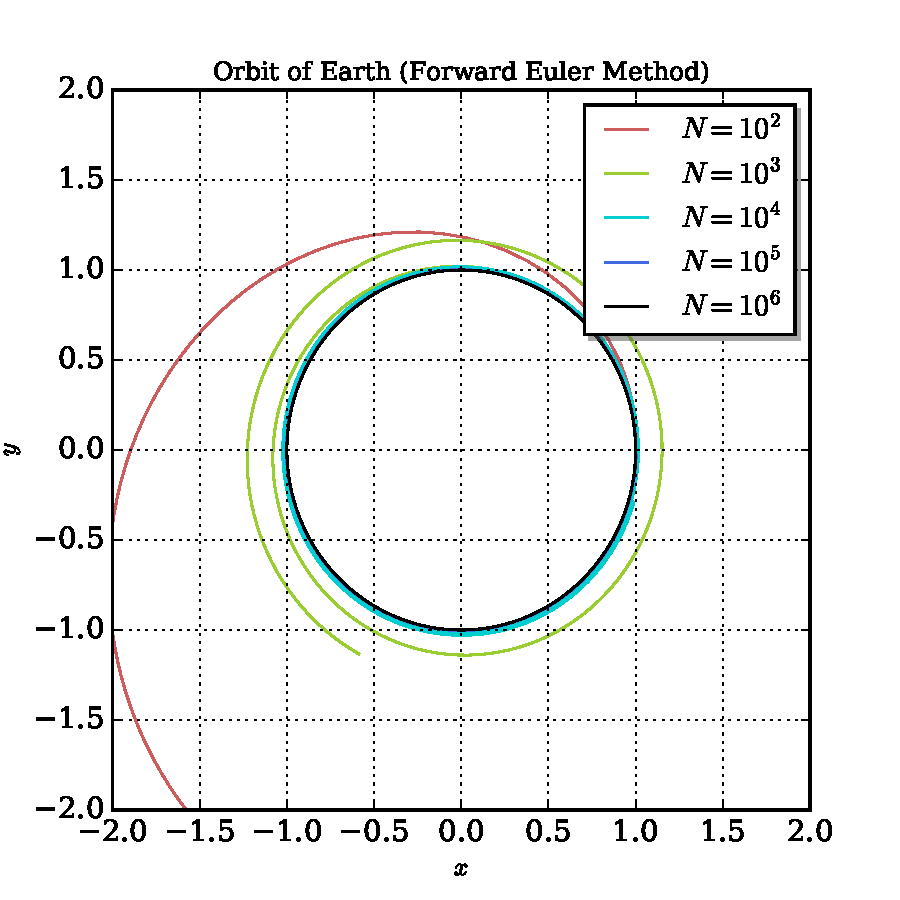
\includegraphics[scale=0.7]{binary_euler_orbit.pdf}
\end{figure*}
\end{center}




\newpage 
\begin{references}
\bibitem{notes} M. Hjorth-Jensen. "Computation Physics, Lecture Notes Fall 2015". University of Oslo. August 2015.
\end{references}

\end{document}
